\documentclass[a4paper]{refart}
\usepackage{graphicx,array,tabularx,pdfpages}
% http://tex.stackexchange.com/questions/124836/full-width-table-with-caption-in-refman-doc
\newenvironment{fulltable}[1][tbp]
 {\begin{table}[#1]%
  \hspace*{-\leftmarginwidth}%
  \begin{minipage}{\fullwidth}}
 {\end{minipage}\end{table}}

\begin{document}
\title{SFMP Baseline Survey Enumerator Training}

\maketitle

Wherever was possible, this manual uses verbatim sections from \textit{Feed the Future (FtF) Population based Survey in Northern Ghana Enumerators' Manual}.

\section{Survey}

\textbf{NOTE: NEARLY ALL QUESTIONS ON THE SURVEY FORM ARE REQUIRED - THE SURVEY CANNOT BE SUBMITTED UNLESS VALID ANSWERS ARE ENTERED FOR EACH QUESTION. DO NOT SKIP ANY QUESTIONS.}

\textbf{NOTE: ALL SURVEYS ARE TO BE ADMINISTERED TO FISHING-DEPENDENT HOUSEHOLDS ONLY! If a household coordinate corresponds to a household which does not participate in fishing activities, you must take note of this and move on to the next household coordinate.}


\subsection{Definition of a Household (from Feed The Future)} 

A household consists of a person or group of related or unrelated persons, who live together in the same housing unit, who acknowledge one male or female as the head of the household, who share the same housekeeping and cooking arrangements, and are considered as one unit. 

Remember  that  not  all  related  persons  living  in  a  house  form  one  household,  and  that  more than one household may live in the same house but one household cannot live in two different houses. A group of people living together in the same house, but each with a separate eating arrangement should be counted as separate one-person households. Please, probe well to put every person in the right household. 
The following examples can be helpful to put persons found in a house or compound into the right households:
\begin{enumerate}
\item In general, a household consists of a man or a woman, with a spouse, children and some other relatives or a house help who may be living with them.
\item In large family houses where there may be two or more generations of relations living, care should be taken not to treat the grandfather, his married children and their families as forming one large household. Note that sharing meals with each other is not the same as sharing the same housekeeping and cooking arrangements. Probe well to separate the various households.
\item Treat as one household if a man lives with more than one wife and their children in the same house and eats successively with each of the wives in turns.
\item If a man does not live in the same house as his wife or wives, the man and his wife/wives must be considered as separate households. Any children and others must be included in the household of the one in whose house they sleep. Thus, if a man and his wife live in different houses and their two sons sleep in the father's house after eating in their mother's house, the children must be included in the father's household while the mother is listed as a single-person household.
\item A house help and his family who live in a house or an out-house in the same compound as the employer must not be included in the employer's household if they prepare their own food. However, if they eat and sleep with the employer, they should be considered as part of the employer's household.
\item If two or more unrelated persons live together in one room or apartment, they should be considered as separate single-person households if they do not share a common catering arrangement.
\item A lodger (or percher) who has stayed with the household for a period of 6 months or more and shares the same cooking and housekeeping arrangement with the household should in this sense be regarded as a member of the household. This should be the case even if the individual expresses an intention to leave soon or in the future.
\end{enumerate}

\subsection{Household Identification (A)}
\textbf{This section is filled out for every respondent. These questions are designed to be filled out through enumerator observation and simple inquiries.}


\begin{description}
\item[A 1.01 Enumerator Identifier] This is the code assigned to you, the enumerator. Type it in for each survey form you fill out. This will be the same number each time you complete a form.

\item[A 1.02-4] Select the region/district/community you're conducting the survey in.

\item[A 1.05] Type in the number of the coordinate (from the Map application) that you're attempting to survey. For example, is this survey location 1? Location 23? Ideally, you will conduct two interviews per location - one for the Head of Household and one for the Gender-Opposite Seniormost Member. Each interview's survey form will have the same number in this field.

\item[A 1.06] Status of location. If none of the options apply, select OTHER and type out the issue in the text field. If multiple households reside within the same structure, enter the number of total households and use the random number booklet to select the household to interview:
\begin{itemize}
\item Order the households (arbitrarily). For example, if there are four households within the structure, assign the number 1 to a household, 2 to a different household, 3 to another, and 4 to the last. The ordering does not matter, but should be noted somewhere so that it does not change.
\item Look at the column in the random number booklet which contains the number of households in the structure.
\item The top-most available number is the random household which you will attempt to survey (for both the Head of Household and Gender-Opposite Seniormost Member). If this household does not participate in fishing activities, you must move on to the next coordinate.
\item Cross out the number you just used. The next time you need to use this column in the random number booklet, the number below the one you just crossed will be the top-most available number.
\end{itemize}

%\item[A 1.07 Type of Household]

%\item[A 1.08 Main Religion of Household]

\item[A 1.09 GPS Coordinates] Populate the fields using the tablet's GPS by clicking the icon shown below. If the accuracy field is above 100m, re-populate the fields by pressing the button again. The accuracy can be improved by doing this in view of the sky outside of the structure.

\includegraphics[width=\textwidth]{enketo2.png}

%\item[A 1.10 Main Ethnic Group]

\end{description}

\subsection{Informed Consent}
Read out the consent form to the respondent and make sure that they understand the contents of the form. If they agree, ask them to sign form to indicate their consent. Only after the respondent signs (or refuses to sign / does not consent) should you continue filling out the survey form.

If the respondent does not consent to the interview, mark this on the survey form and select SUBMIT to complete this form.

\includegraphics[width=\textwidth]{consent.png}

If the respondent consents to the interview, record their name in the text field. If the respondent has a mobile number which they may be reached at, record it in the next text field.


\subsection{Household Demographics (B)}
\textbf{These questions are administered for all respondents and are targeted towards the specific individual being interviewed. Remember to note the respondent's age in COMPLETED years (i.e., their age at their last birthday)}

\begin{description}
\item[B 1.01 Role in household] Head of Household refers to the person who the majority of the household acknowledge as responsible for household-wide decisions. This is often the male in households containing a husband and wife. The Gender Opposite Seniormost Household Member is the OPPOSITE gender as the Head of Household (i.e. if the Head of Household is a MALE, this must be a FEMALE in the household) and refers to the person who is the closest counterpart to the Head of Household (regarding household-wide decisionmaking). This could be the spouse of the Head of Household, an elder figure in the household, or one of the oldest children.

\item[B 1.06 Attended school] School refers to formal schooling or attendance of either a Primary, Middle/JSS, Secondary school, Vocational/Technical, Professional school or Training, Polytechnic, or a University. Attendance at a Koranic school, for no matter how many years, is not to be included.

\item[B 1.06A Highest qualification] The ``highest qualification of education completed'' means the highest level of formal schooling completed. If someone dropped out of school at a level it means he/she has not completed that level and so it should not be recorded as the highest. For instance, a drop out from secondary school form three during the second term will have his/her highest educational level completed to be probably the MSLC/JHS level since he could not finish the secondary school.

\textit{Note:}

\textit{TECHNICAL AND PROFESSIONAL TRAINING} includes, for example, courses in accounting, secretarial courses, training in the POLYTECHNICS, I.S.S.E.R., School of Journalism, and so on. This does not refer to on-the-job training.

\textit{TECHNICAL OR PROFESSIONAL CERTIFICATE} refers to a certificate received from such types of training institutes like technical and advanced/specialist colleges. Certificates awarded by such training institutes include the following: an advanced/diploma, a state registered nurse's certificate and others.

\textit{TECHNICAL OR PROFESSIONAL DIPLOMA} refers to a diploma received for the successful completion of the appropriate level of training, for example, a diploma in statistics, etc.

\end{description}

\subsection{SFMP Questions (C)}
\textbf{These questions are administered to all respondents}
\begin{description}

% NEED TO DEFINE MEANING OF LIKERT ITEMS

% Increased a lot
% Increased somewhat
% Stayed about the same
% Decreased somewhat
% Decreased a lot

% All the time
% Frequently
% Rarely
% Not at all / Never




\item[C 1.01 Livelihood activities] If at least one answer is selected, the respondent will have to answer which of the engaged activities is the most important to the household (C 1.01C). If at least two answers are selected, they will also have to answer which is the secondmost important (C 1.01D). These answers should coincide with the answers to C 1.01 and should not conflict with one another (do not mark the same activity as both the most and secondmost important)

%\item[C 1.02 - 1.09 Compared to 5 years ago...] All of these questions are aimed at assessing if there has been a change from five years ago, and if so, in what direction.


\item[C 1.15 Illegal fishing activities] If at least one answer is selected, the respondent is asked which is the most frequent violator (C 1.15A). The answer to the followup question should not conflict, that is, the most frequent violator should not be an answer that was not checked in C 1.15.

\end{description}

\subsection{Household Hunger Scale (D)}
\textbf{This section will only appear if the respondent was marked as ``Head of Household'' in the Household Demographics section.}

D 1.01 asks whether over the past 4 weeks, there ever was no food to eat of any kind in the house because of lack of resources to get food. It is important to note that this is different from somebody skipping a meal due to illness, lack of taste, etc. It refers to one, some or all members of the household skipping or failing to get food to eat due to insufficiency or unavailability. The reference period is the past 4 weeks prior to this interview.

Although there are pre-coded response options, these should be read only for the first HHS question, as suggested response options. The respondent should be allowed to answer in his or her own words. The enumerator will then select the most appropriate response option based on the respondent’s reply. If the respondent has difficulty replying, then the interviewer can encourage a response by listing the set of options again.

Table \ref{hhstable} gives the intended meaning of key concepts in the questions that should be taken note. In case of translation into any local language, the enumerator should make sure that all the intended meaning is conveyed in the translation.

\begin{fulltable}
\begin{tabularx}{\textwidth}{| X | X |} \hline
HHS Question & Intended Meaning of HHS Question \\ \hline \hline
D 1.01 No food of any kind in the house &
This question asks about a situation in which there is no food to eat of any kind in the house because food was not available to household members through usual means (e.g. through purchase or barter, gifts from the garden or field. from storage structures) \\ \hline
D 1.02 Go to sleep hungry because there was not enough food &
This question asks whether the respondent or other household members felt hungry at bedtime because they did not have enough food to eat during the day and evening.\\ \hline
D 1.03 Go a whole day or night without eating & 
This question asks whether any household member did not eat from the time they awoke in the morning to the time they awoke the following morning because there was not enough food. A person who chooses not to eat for a whole day for reasons other than lack of food (for example, if fasting or on a diet) should not respond affirmatively to D 1.03. \\ \hline
Food (all questions) &
The word ``food'' may be synonymous with the major staple food in some cultures. The use of the word ``food'' in the Household Hunger Scale, however, means all foods, i.e., anything that is edible, not just the staple starch. It may be possible that a household that is unable to get the staple \textit{Tuo Zaafi} may count that as not having eaten even if they are able to get some bread to eat. \\ \hline
House ( D 1.01 ) &
asks about the availability of food in structures belonging to the household (i.e., the house itself and any storage structures). \\ \hline
Lack of resources ( D 1.01 ) &
``Lack of resources'' refers to the lack of money to buy food or the inability to produce or barter for food. \\ \hline
Hungry ( D 1.02 ) &
To be “hungry” is to have a compelling need or desire for food, to have a painful sensation, or to be in a state of weakness caused by the need for food. A hungry person is not necessarily one who has not eaten at all; food eaten may not have been enough to fill the belly. \\ \hline
\end{tabularx}
\caption{HHS Definitions}
\label{hhstable}
\end{fulltable}

\subsection{Women's Dietary Diversity}
\textbf{This section will only appear if the respondent was marked as ``female'' in the Household Demographics section and the respondent's age was recorded as 49 years or younger.}

Whilst woman tells you of the foods that she ate the whole day and night, mark each food group as a relevant food is mentioned. Allow the  woman to describe the foods and liquids that she ate or drank yesterday, during the day or night (from time of wake-up till went to bed) whether at home or outside the home. When dishes are mentioned, ask what the ingredients in the dish were so the appropriate food groups can be marked. It is only necessary to mark the food group the first time one of the applicable foods in the group is mentioned.

\textbf{Note: The reference period to all these questions is YESTERDAY}

\subsection{Dwelling Characteristics (F)}
\textbf{This section will only appear if the respondent was marked as ``Head of Household'' in the Household Demographics section.}

The respondent should be the person who is most knowledgeable about the dwelling characteristics and its ownership arrangement in the household.

Definitions
\textit{Dwelling:} This includes all types of structures occupied by members of a household. These may consist of a house, a room inside a house, a group of houses, a multi-storeyed house, and a hut or group of huts.

\begin{description}
\item[F 1.01-04] You are to observe the house or the structure and record your observation. Even when the interview is conducted in a place outside of the household dwelling, the enumerator should visit the dwelling to make these observations. However, if the interview is conducted outside of the dwelling and there is no chance to observe the floor material, then this could be asked. Where different portions of the dwelling are constructed of different types of materials, the enumerator should record the dominant material for each of the questions.
\item[F 1.05-08] These questions ask about the utilities and amenities of the household. Access to electricity is irrespective of the source so far as there is power: whether connected to the national grid, powered by a generator or relies on solar panel power generation. However, a wired house with non-connected or disconnected power source should not be recorded as having access to electricity. Regarding the main source of cooking fuel for the household: select OTHER in the case where no cooking is done in the household.
\end{description}

\subsection{Women's Empowerment in Agriculture Index (modified) (G)}
\textbf{This section is administered to all respondents, not just women.}

This module should be conducted strictly under private, where other members of the household cannot overhear or contribute answers. Do not attempt to make responses between a primary and secondary respondent the same. Ensure that you code the outcome of the interview at the end of interview for each target respondent.


\textit{Purpose}
The purpose of this module is to get an idea about men's and women’s relative roles in decision making around income-generating activities. Do not attempt to ensure that responses are the same between the male and female respondent. It is okay for them to be different.

\subsubsection{Role in Household Decision-making around production and income generation}
\begin{description}
\item[Did you (singular) participate in\ldots]
Note the following:
In some languages there is a singular ``you'' and a plural YOU. The individual level question refers to the singular you (the person being interviewed, not the respondent together with his or her family). The respondent needs to understand that this applies to just him/her.
In some cases, for crop production related activities, it will be helpful to ask the respondent to think about the last cropping season or two cropping seasons if the area has a bi-annual crop season.
\item[Contribution / Role in making decisions] Note that whilst the first concerns decision about production, the second relates to decisions on the use of income generated from the [ACTIVITY]. Also note that the two questions are answerable using the same codes. NO DECISION MADE however should be entered in the case that the decision is not made. This also fits a situation where crops have been lost in a cropping season so no income was generated or livestock/livestock products were not sold so income was not generated.
\end{description}

In some cases respondents will need more explanation about what certain categories contain. In this case the enumerator can use simple examples tailored to specific activities undertaken by households in the survey area to explain.
Examples can be:
\begin{description}
\item[Food crop farming:] crops that are grown primarily for household food consumption: For example, did you have input into decisions about what crops to plant this year or in which plots they would be planted, or which seeds, fertilizer (other inputs) your family would buy?
\item[Cash crop farming:] crops that are grown primarily for sale in the market: For example, did you have input into decisions about how much of your family's land would be used for growing cash crops, or about the crops to be grown for sale, and the inputs to be used for those crops?
\item[Livestock raising:] For example, did you have input into decisions about the purchase, care, or sale of livestock?
\item[Non-farm economic activities:] Small business, self-employment, buy-and-sell: For example, did you have input into purchases made for a small business or goods sold?
\item[Wage and salary employment:] in-kind or monetary work both agriculture and other wage work: For example, did you have input into decisions about if you or other household members will work outside the home?
\item[Fishing or fishpond culture:] For example, did you have input into decisions about when to do fishing, or how to stock a fish pond, inputs for fish culture?
\end{description}
In the case that a crop is grown partially for food and partially for sale on the market, record that activity only once, in the category which the crop is primarily grown for (in terms of volume).

\subsubsection{Access to Productive Capital}
The purpose of this module is to get an idea about men's and women's access to capital or assets and their ability to control use of the resource. Again, do not attempt to ensure that responses are the same between the male and female respondent.
The questions ask about men's and women's access to different types of assets and ask about different types of decisions on each type of asset, and who makes those decisions most of the time.

It is most preferred that the questions are asked for all assets before asking the sub questions. That is, ask G 1.07, then G 1.08 (skipping G 1.07A,B,C even if the respondent answers YES to G 1.07) until all YES/NO questions in this module have been answered. In this way, respondents have no incentive to undercount assets because of the perception of having to answer the remaining sub questions.

After asking all YES/NO questions, ask all the sub questions for one type of asset at a time before going to the next type of asset so that the respondent is consistent in answers across the types of decisions. (that is, ask G 1.07A,B,C before moving to G 1.08A,B,C, etc).

It is important not to double count assets into two categories when thinking about different asset categories. For example, it is important to distinguish between large livestock and small livestock; Farm equipment (non-mechanized), Farm equipment (mechanized) and Nonfarm business equipment; clearly beforehand so that respondents do not add all together and later have to answer same for subsequent options.

Non-farm activities include any asset used for small businesses including solar panels (if used for recharging), sewing machine, brewing equipment, frying equipment, etc. The distinguishing factor between farm and nonfarm activities is the value addition to production (i.e. Brewing or processing like baking bread).

Note: Items which are not functioning at the time of interview are to be counted insofar as there is a resale value for the asset (i.e. it can be fixed or it can be sold to buy another productive asset or service).

Also NOTE that questions referring to ``general'' decisions or who takes decision on the items mean MOST OF THE TIME. The codes for all these questions are the same.


\subsubsection{Access to Credit}
This module seeks to get an idea about men's and women's access to credit. Do not attempt to make responses from the two respondents the same.
The questions ask about men's and women's access to sources of lending credit, who makes the decision to borrow or not to borrow from a particular source, and decision on the use of the credit.

It is possible that other individuals in the household access credit that may not be known to the respondent. In that case the response DON'T KNOW can be entered.

NOTE that the reference period for the module is the past 12 months.

\textit{Lending source names}
\begin{description}
\item[NGO] As known to the respondent. Where the category of the lending source is not clear, the enumerator should note this and discuss with the supervisor for verification.
\item[Informal lender] This include any local money lender who charges interest on loans given
\item[Formal lender] As known to the respondent
\item[Friends or relatives]  As known to the respondent
\item[micro-finance/VSLAs/susu]  As known to the respondent.
\end{description}

\subsubsection{Individual leadership and influence in the community and Group Membership}
The purpose of these modules are to get an idea about men's and women's potential for leadership and influence in the communities where they live. Again, do not attempt to ensure that responses are the same between the male and female respondent.

\subsubsection{Decision Making}
The purpose of this module is to get additional information about decision making within households. These questions are different from the previous questions on decision making, because we are now asking whether the respondent is satisfied about decisions made, and motivations for making these decisions.


\section{Equipment}
The survey is being conducted on SAMSUNG tablets, using the Enketo Smart Paper system. The survey forms are filled out using the Chrome web browser.

Surveys are to be administered at pre-specified locations. The locations are available via Google Maps as well as the offline SFMPSurveyApp, both available on the tablets. These three applications, Google Maps, SFMPSurveyApp, and Enketo (through Chrome) are stepped through below.

\includegraphics[width=\textwidth]{applauncher1.png}


\subsection{Google Maps}
After launching the ``Maps'' application, you should see your position indicated as a blue dot on the map. It may take a minute or two for the position to stabilize. Click the button in the corner to center the map on your location (and zoom in slightly if necessary).

\includegraphics[width=\textwidth]{googlemaps1.png}

Use the icon on the left to open the menu containing ``My Places'' to display the sample locations for a given community on the map.

\includegraphics[width=\textwidth]{googlemaps2.png}

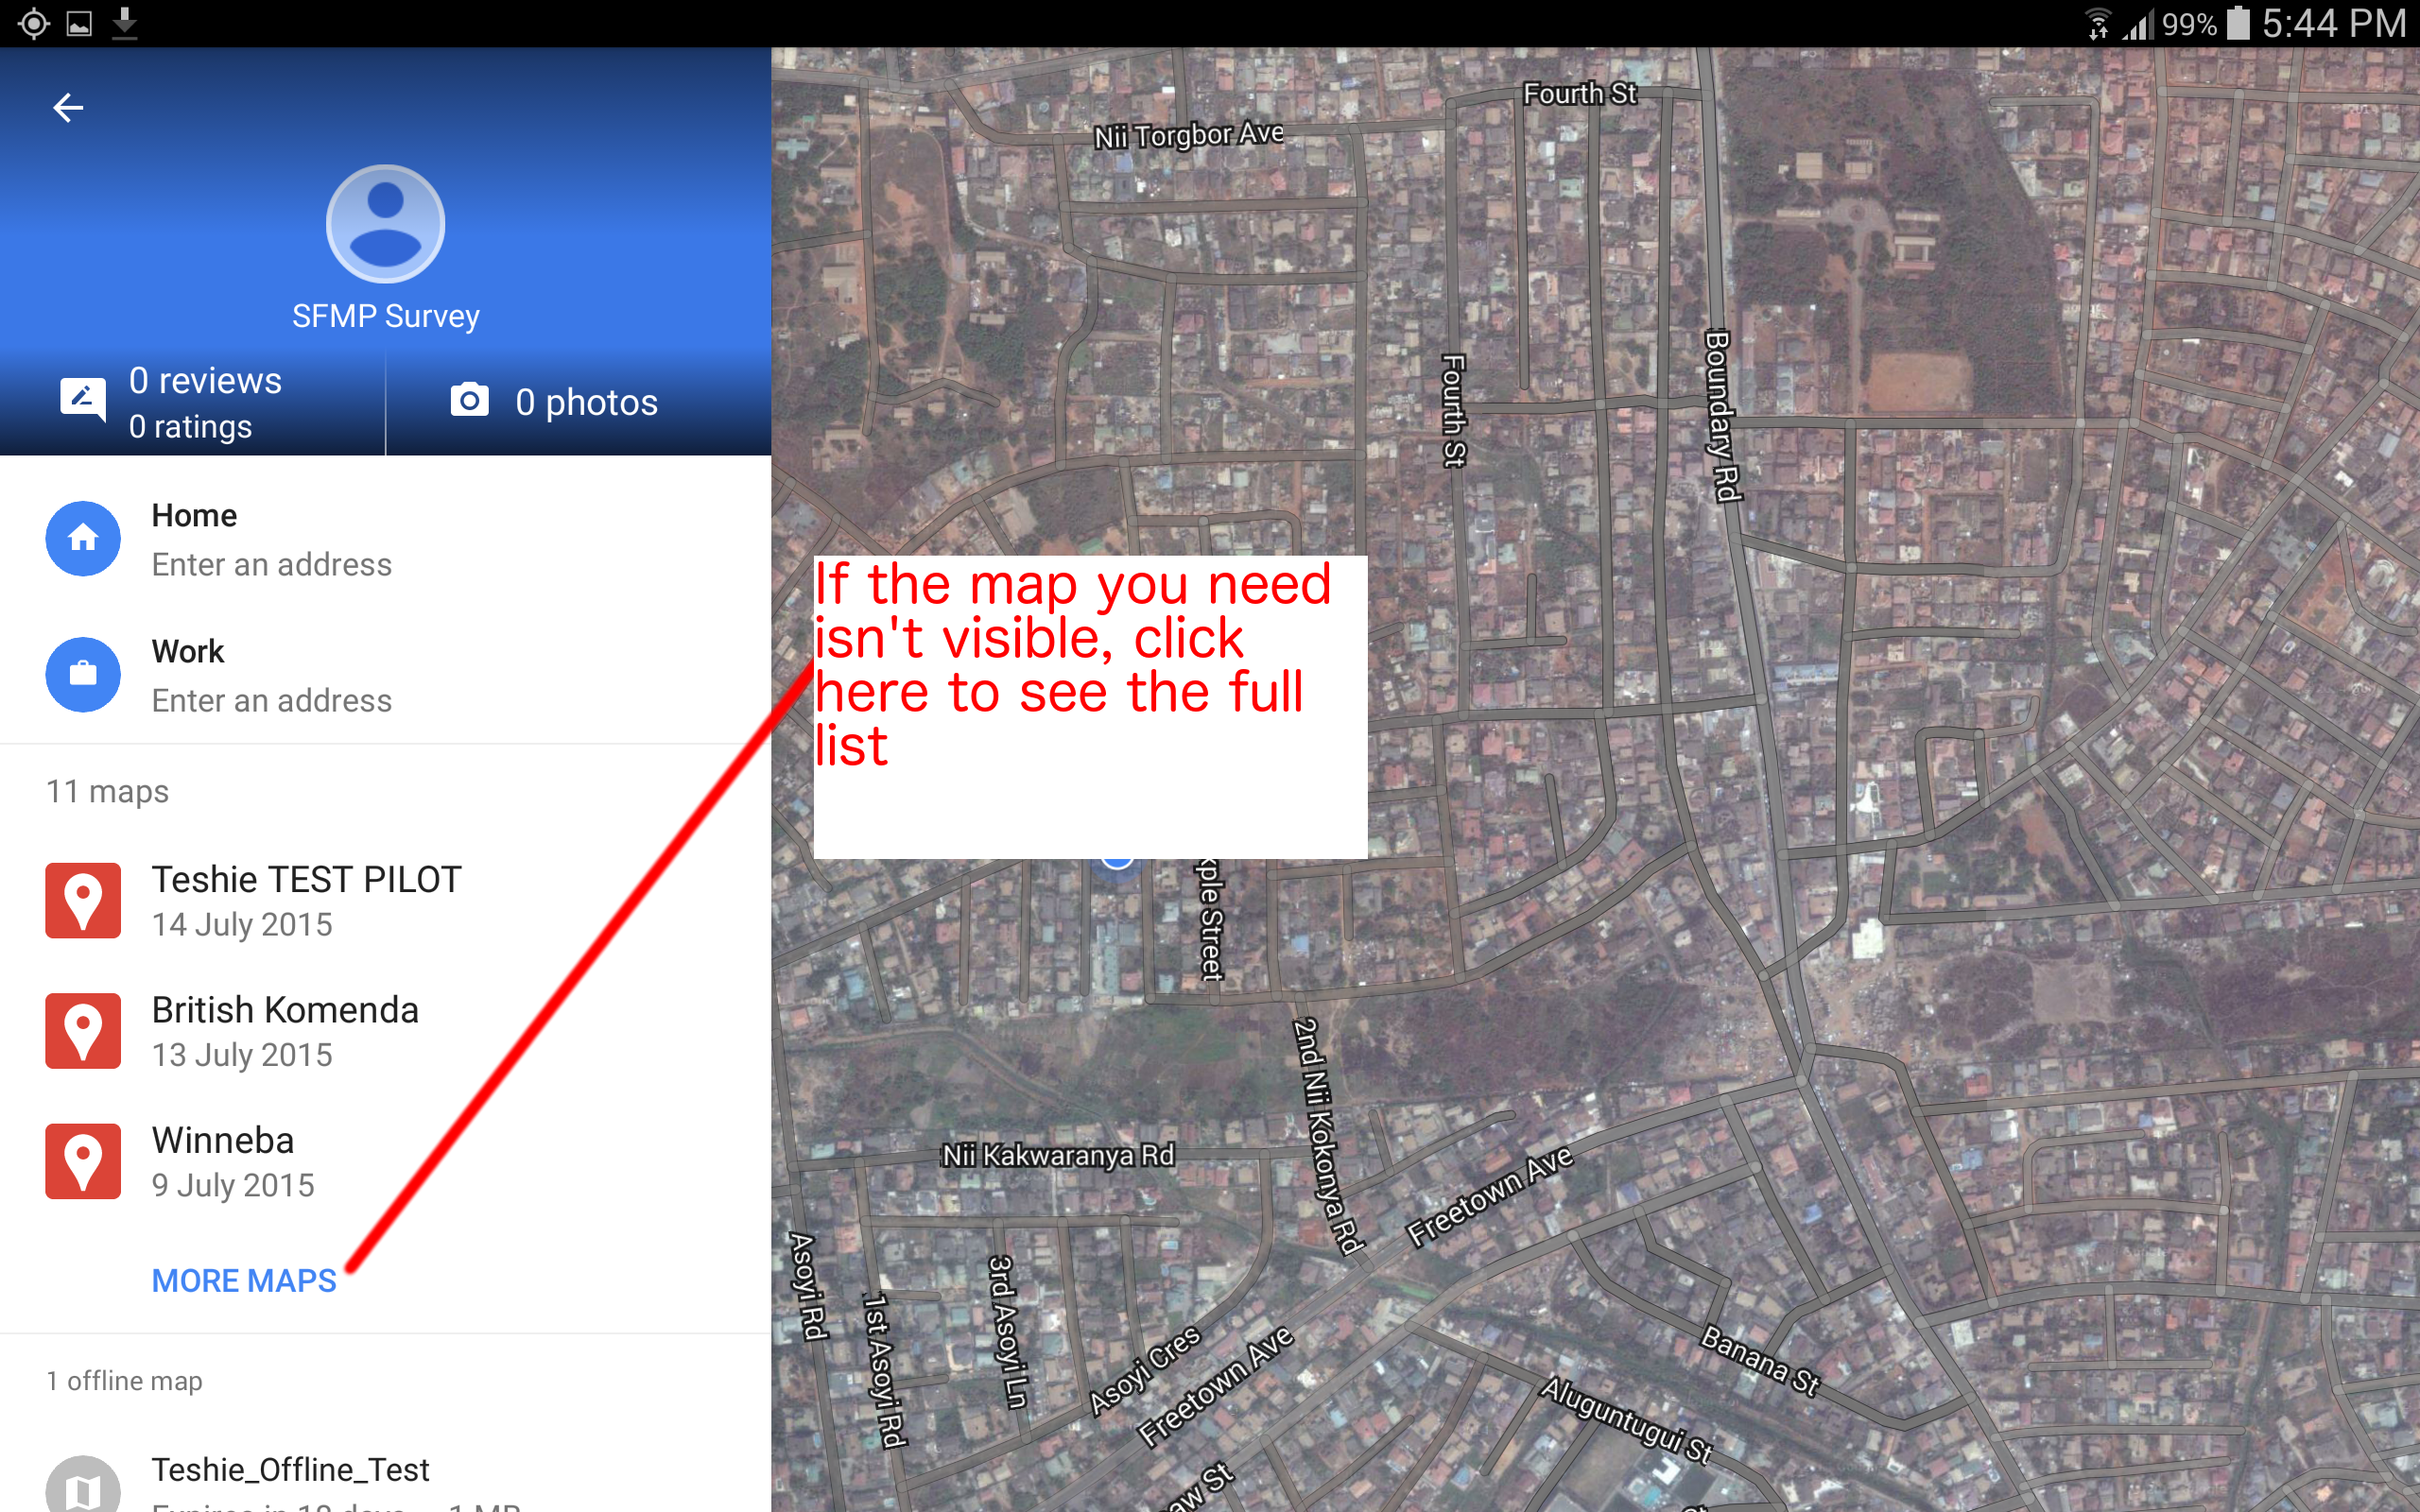
\includegraphics[width=\textwidth]{googlemaps3.png}

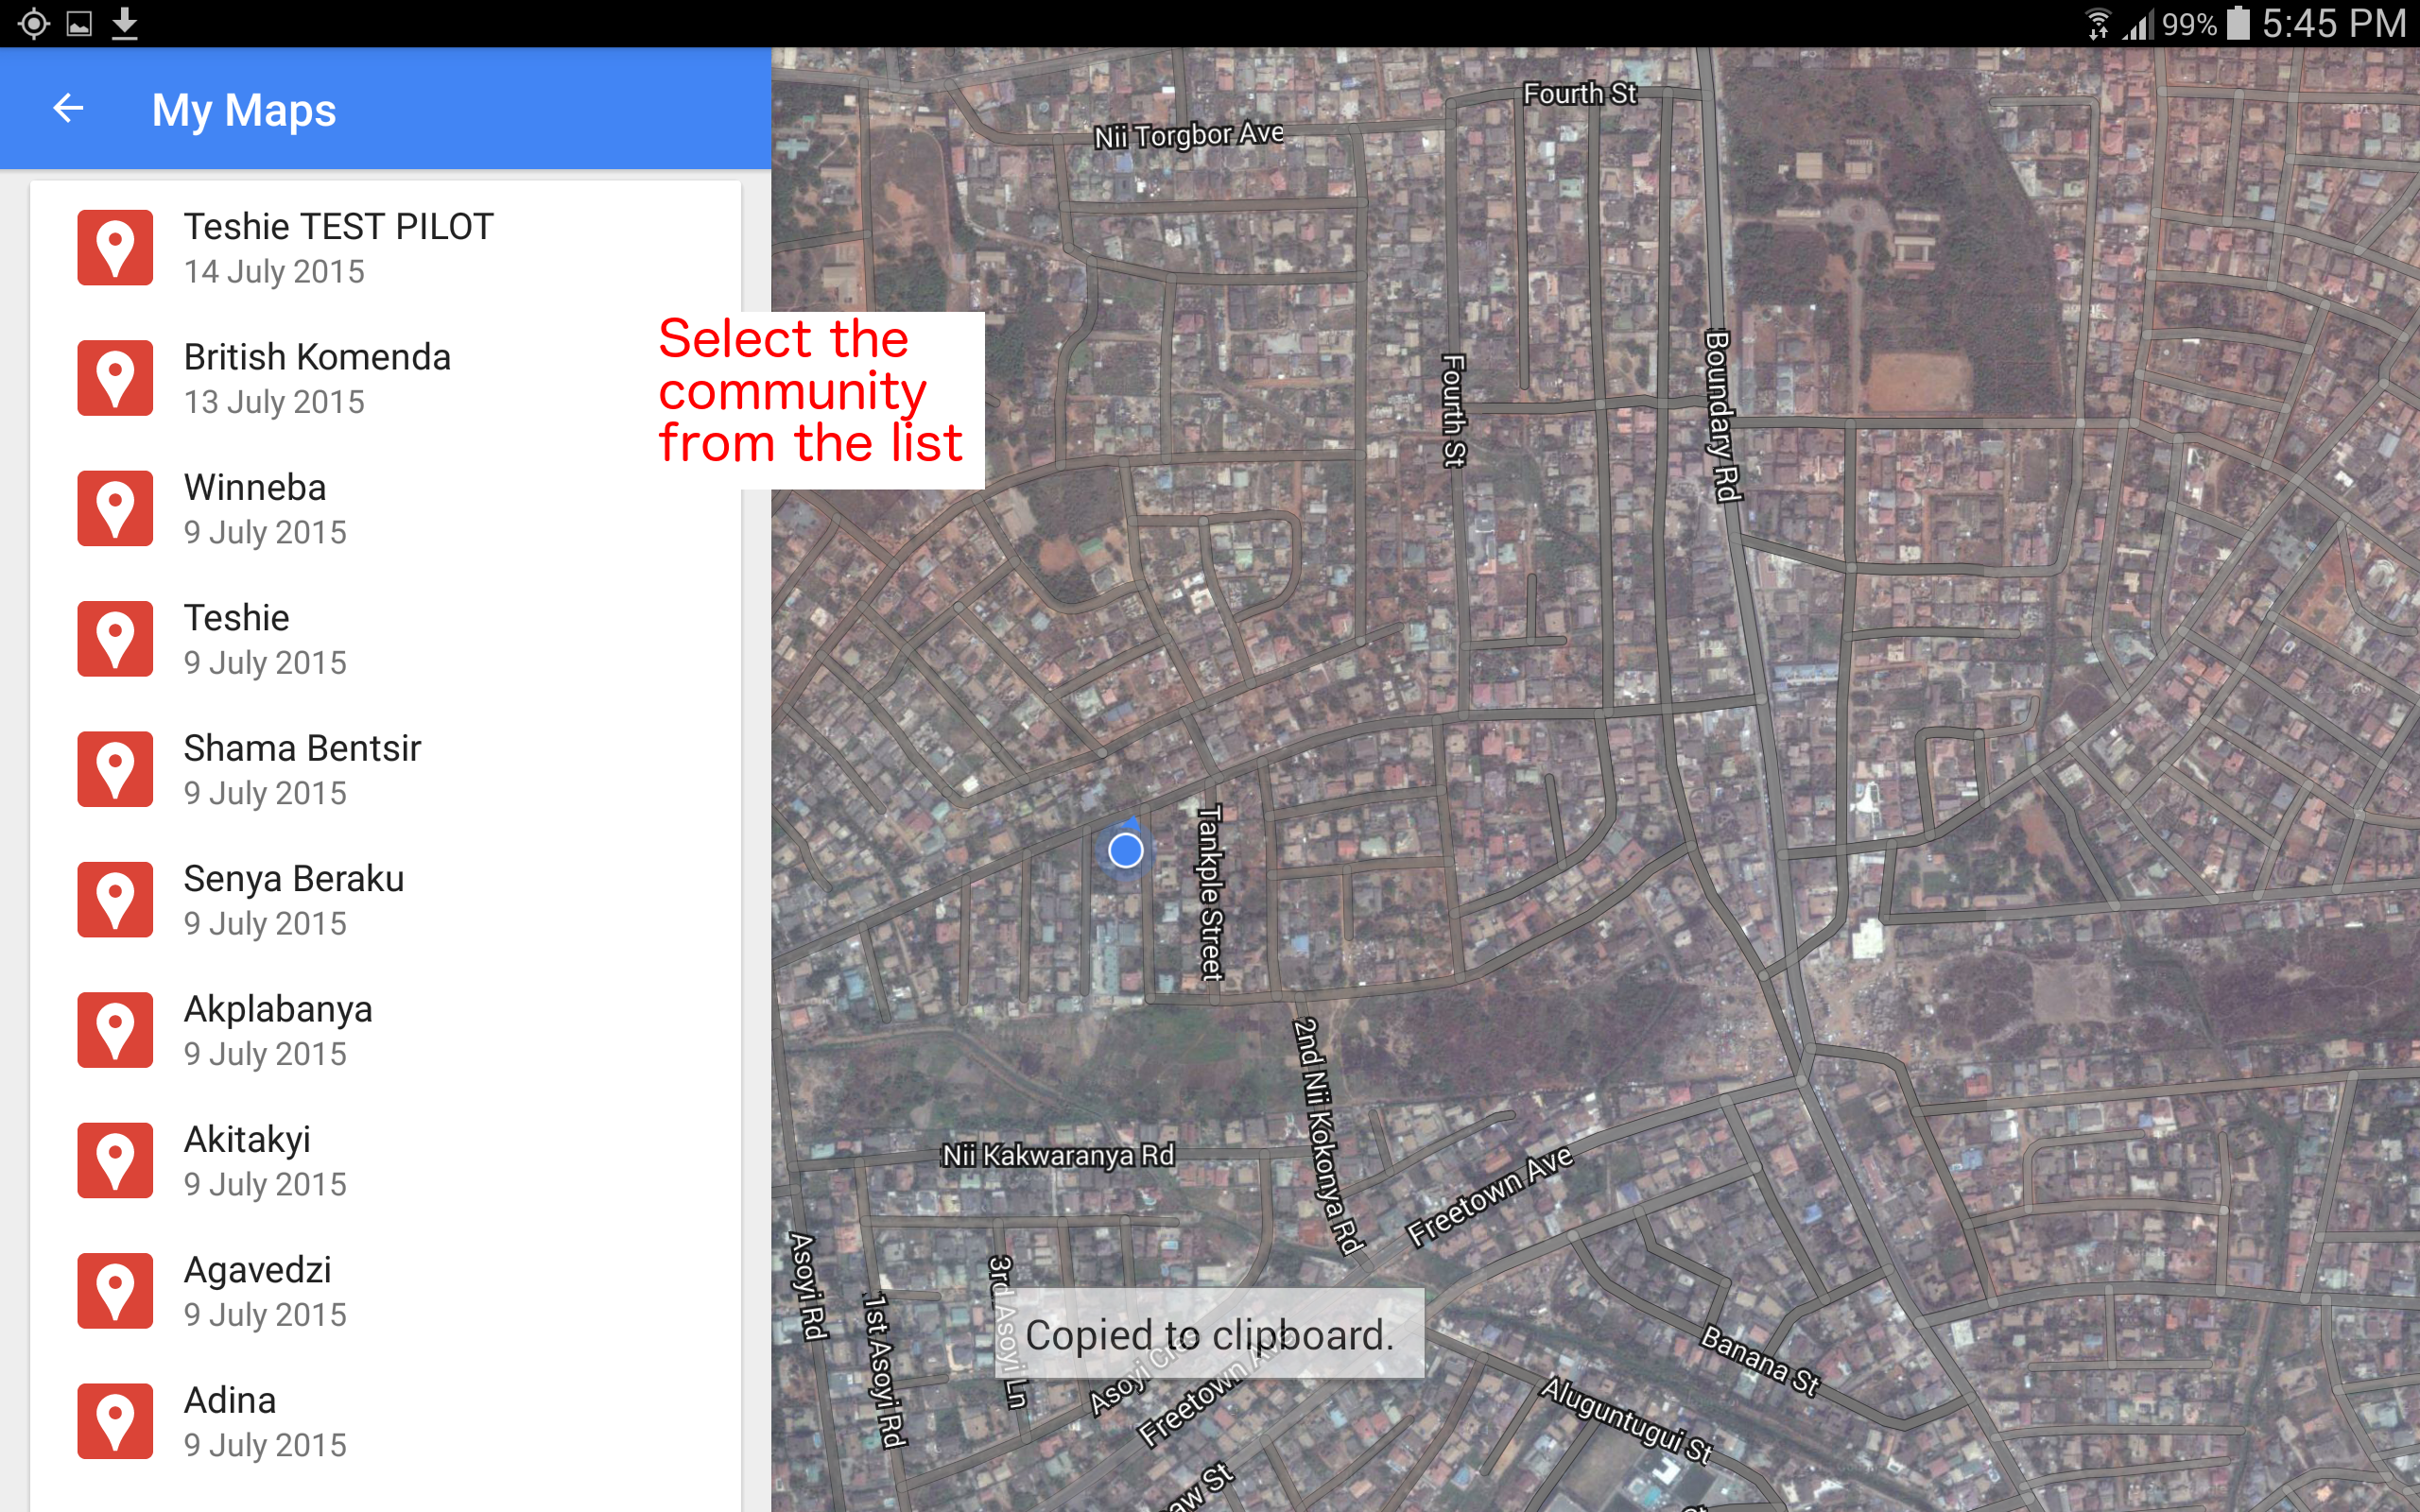
\includegraphics[width=\textwidth]{googlemaps4.png}

The icons represent GPS coordinates to conduct the survey at. Green icons are survey points and orange points are backup points to be used at the discretion of the field coordinator.

\includegraphics[width=\textwidth]{googlemaps5.png}

Additional information can be obtained by clicking on either ``view map legend'' or on a particular sample point.

\includegraphics[width=\textwidth/3]{googlemaps6.png} \includegraphics[width=\textwidth/3]{googlemaps7.png}


\subsection{SFMP Baseline Survey App}
After launching the ``SFMPSurveyApp'' application, you should see your location displayed on a map of the surroundings.

\includegraphics[width=\textwidth]{sfmpapp1.png}

Click the ``Show List of Communities'' text to display the list of survey communities, and click on the text of a community to display the survey coordinates related to that community.

\includegraphics[width=\textwidth]{sfmpapp2.png}

The GPS locations are shown with icons. Green icons are locations to be surveyed and orange icons denote backup points to be used at the discretion of the field coordinator.

\includegraphics[width=\textwidth]{sfmpapp3.png}

Buttons at the bottom of the app allow you to center the map at your position, toggle the display of the icons, or select a particular survey point by number.

\includegraphics[width=\textwidth/2]{sfmpapp4.png}
\includegraphics[width=\textwidth/2]{sfmpapp5.png}



\subsection{Enketo (and Chrome)}
After launching ``Chrome'' and opening the Survey URL, you should see an empty survey form.

\includegraphics[width=\textwidth]{enketo1.png}

The buttons at the bottom of the form allow you to move around the survey. You can move forward one page (NEXT), back one page (Back), Jump to the first page, or jump to the last page.

\includegraphics[width=\textwidth]{enketo3.png}

On the last page of the form, (NEXT) turns to (SUBMIT). If you have errors with the form and are unable to work through them (after discussing with the field coordinator), select ``Save as Draft'' and click SAVE DRAFT to queue the record for deferred inspection.

\includegraphics[width=\textwidth]{enketo4.png}





\section{Types of Fish and Gear}
The following pages were taken from the \textit{Small Pelagic Fisheries Data Collection: Orientation Training Manual} developed by CRC/SFMP and Hen Mpoano.
\includepdf[pages=-]{orientation_manual_fish.pdf}

\includepdf[pages=-]{orientation_manual_gear.pdf}

\end{document}